\documentclass{beamer}
\usepackage{ctex, hyperref}
\usepackage[T1]{fontenc}

% other packages
\usepackage{latexsym,amsmath,xcolor,multicol,booktabs,calligra,color}
\usepackage{graphicx,pstricks,listings,stackengine,subfigure}

\author{Can Xu}
\title{Self introduction and future plans}
\subtitle{}
\institute{}
\date{2023/6/17}
\usepackage{zjgsu}
\setsansfont{Times New Roman}
\setmainfont{Times New Roman}

% defs
\def\cmd#1{\texttt{\color{red}\footnotesize $\backslash$#1}}
\def\env#1{\texttt{\color{blue}\footnotesize #1}}
\definecolor{deepblue}{rgb}{0,0,0.5}
\definecolor{deepred}{rgb}{0.6,0,0}
\definecolor{deepgreen}{rgb}{0,0.5,0}
\definecolor{halfgray}{gray}{0.55}

\lstset{
    basicstyle=\ttfamily\small,
    keywordstyle=\bfseries\color{deepblue},
    emphstyle=\ttfamily\color{deepred},    % Custom highlighting style
    stringstyle=\color{deepgreen},
    numbers=left,
    numberstyle=\small\color{halfgray},
    rulesepcolor=\color{red!20!green!20!blue!20},
    frame=shadowbox,
}


\begin{document}

\kaishu
\begin{frame}
    \titlepage
    \centering{}
    % \begin{figure}[htpb]
    %     \begin{center}
    %         
\includegraphics[width=0.15\linewidth]{figure/zjgsu} % 这个位置可能需要调整
    %     \end{center}
    % \end{figure}
\end{frame}

\begin{frame}
    \tableofcontents[sectionstyle=show,subsectionstyle=show/shaded/hide,subsubsectionstyle=show/shaded/hide]
\end{frame}

\section{Basic information}
\begin{frame}{Basic information}
    \begin{itemize}
        \item I'm from Suzhou, Jiangsu.
        \item I got my bachelor's degree at Nanjing University of Information Science \& Technology and currently a master degree candidate of science in Zhejiang Gongshang University.
        \item My github page is \url{https://github.com/LEOXC1571} and my personal blog is \url{https://leoxc1571.github.io/}
    \end{itemize}
\end{frame}

\section{Publications}
\begin{frame}{A fairness-aware graph contrastive learning recommender framework for social tagging systems}
    \begin{itemize}
        \item The proposed method integrates contrastive learning into tag-aware recommender systems. By perturbing features with normalized noises, different perspectives on features are generated. They help the model learn high quality features via contrastive learning tasks.
        \item In order to promote fairness of recommendations, we introduce fairness-aware learning, which jointly optimizes TAGCL through negative tag loss and TransT regularization. Negative tag loss leverages the distribution difference between items and tags in the training data.
        \item TransT regularization is also propsosed to promote consistency between two bipartite graphs. The differences between tag embeddings in separate graphs are regarded as relations between users and items.
    \end{itemize}
\end{frame}

\begin{frame}{A fairness-aware graph contrastive learning recommender framework for social tagging systems}
    \begin{figure}[H]
        \centering
        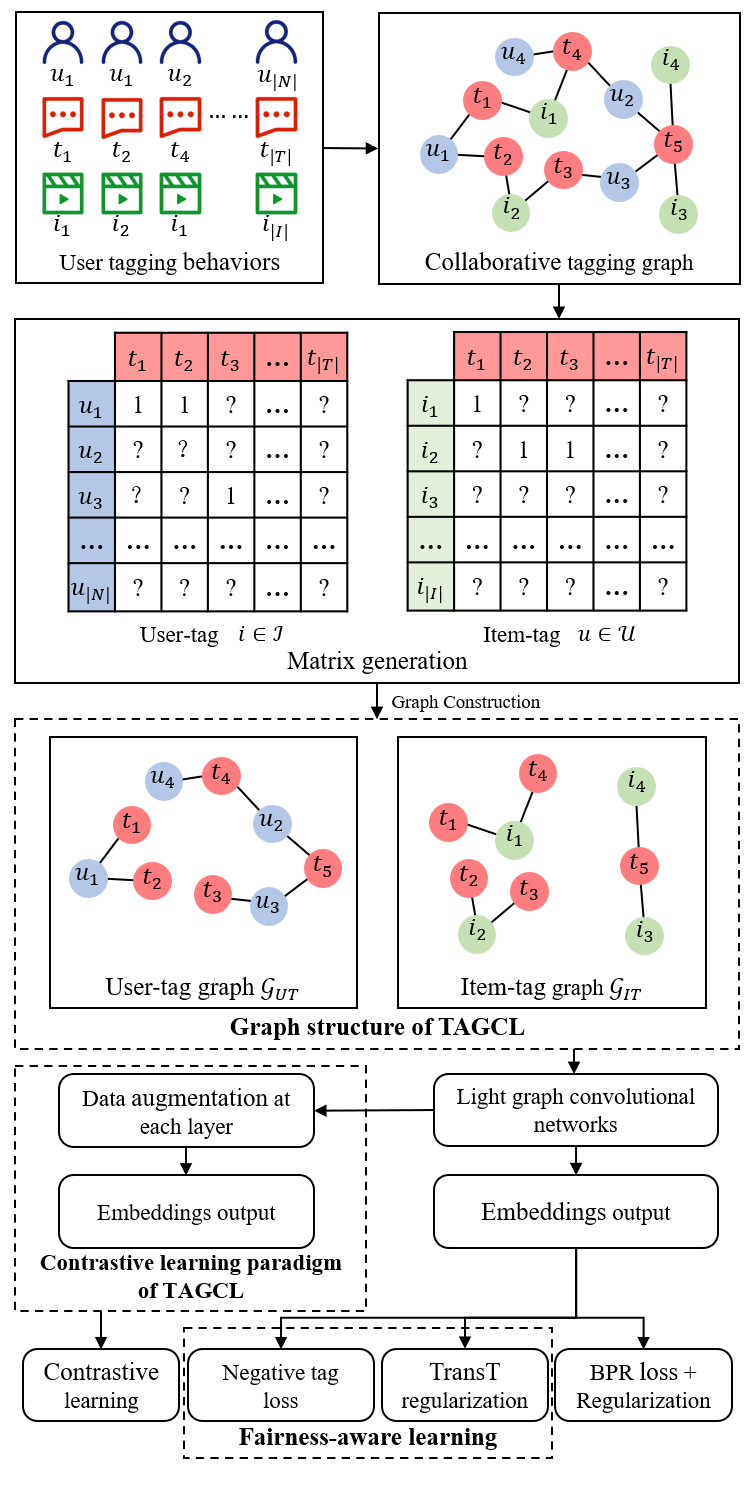
\includegraphics[width=0.28\linewidth]{figure/tagcl.png}
        \caption{Overall structure of TAGCL}
    \end{figure}
\end{frame}

\begin{frame}{A fairness-aware graph contrastive learning recommender framework for social tagging systems}
    \begin{figure}[H]
        \centering
        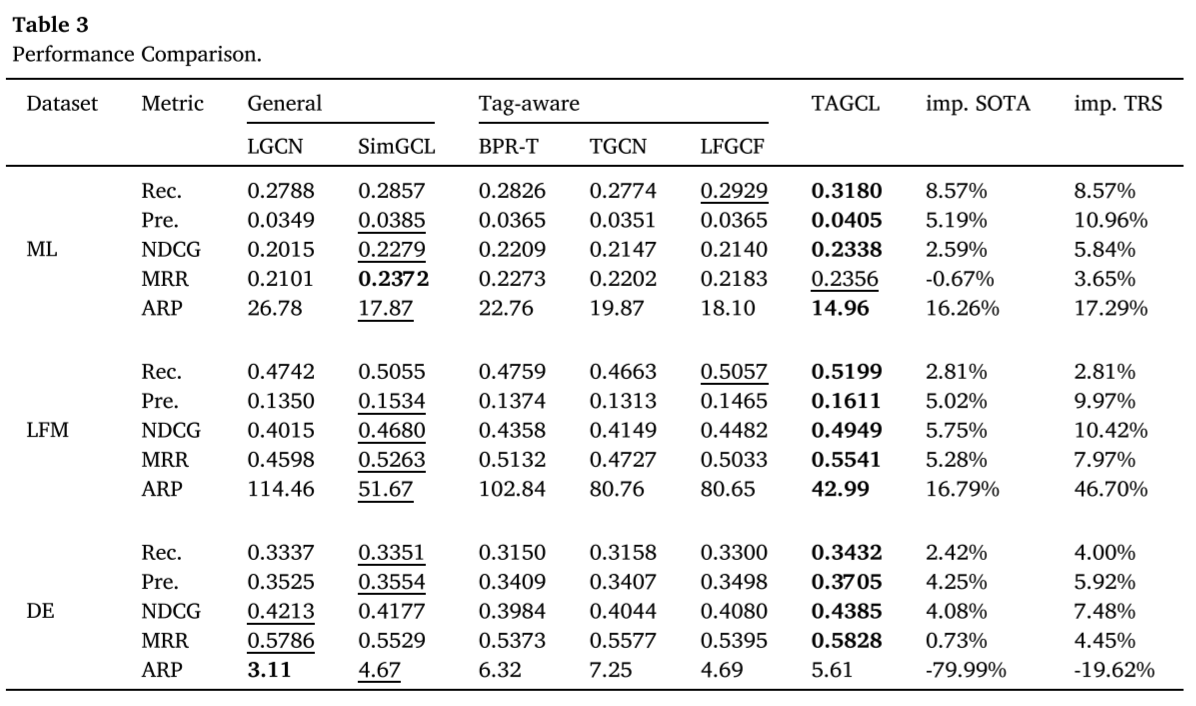
\includegraphics[width=\linewidth]{figure/tagcl_performance.png}
    \end{figure}
\end{frame}

\begin{frame}{Pursuit and Evasion Strategy of a Differential Game Based on Deep Reinforcement Learning}
    \begin{itemize}
        \item For the kinematic solve of dog sheep game, by finding the equilibrium point in the game, this study successfully establishes the kinematic pursuit and evasion policies.
        \item Leverage DQN and DDPG models to train the escaping strategy for intelligent agent.
        \item Propose a refined reward mechanism and an attenuation mechanism to minimize the defect of DQN.
    \end{itemize}
\end{frame}


\section{Experiences}
\begin{frame}{Internship at Zhejiang Lab}
    \begin{itemize}
        \item Working at the research center of graph computing, leading by Hongyang Chen.
        \item Investigate, survey, and repreduce some state-of-the-art large-scale molecular pretraining methods, including MPG, Grover, GEM, MolCLR, and etc.
        \item Compete in OGB-LSC NeurIPS 22, and achieve 11th place at PCQM4M-V2 track.
        \item Patent writing.
        \item Write a survey on diffusion-based graph generative methods.
        \item Propose a diffusion-based 3D molecule generation method.
    \end{itemize}
\end{frame}

\begin{frame}{OGB-LSC NeurIPS 22}
    \begin{itemize}
        \item Propose HFAGNN for large-scale (over 3M) molecular property predictions.
        \item Build up the hybrid block that combines topology and geometry information together. Bessel function is adopted to extract pair-wise and triplet-wise geometric information.
        \item Use multi-gpu training and achieve 11th place of the leaderboard. 
    \end{itemize}
    \begin{figure}[H]
        \centering
        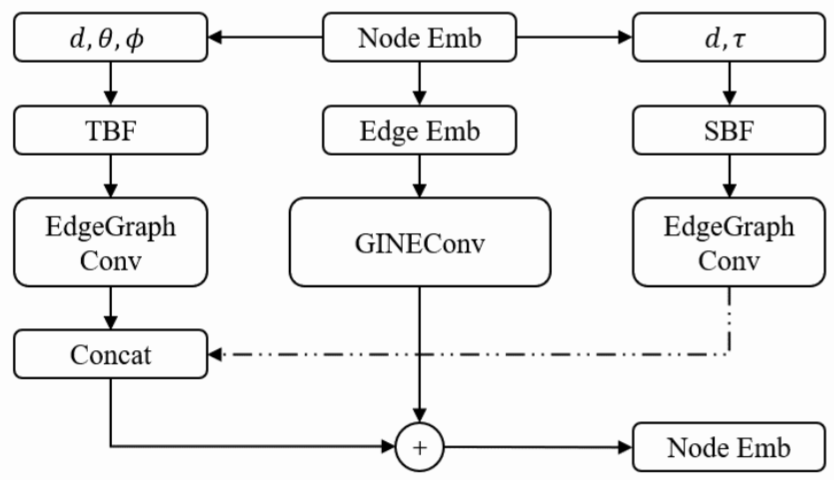
\includegraphics[width=0.6\linewidth]{figure/hfagnn.png}
    \end{figure}
\end{frame}

\begin{frame}{Diffusion-based molecule generation}
    \begin{itemize}
        \item Build up a framework for de novo molecule generation.
        \item Deisgn the E(n) dual-track denoising kernel for effective molecular learning.
        \item The atom-pair track predicts the influence of inter-atomic distances on atomic positions and numbers via global Transformer. Then the pair-wise distance features get updated by the same structure, which incorporates triplet torsion angle information into atom pair features.
        \item Build up a loss function that facilitate correct valencies of atoms.
    \end{itemize}
\end{frame}


\section{Future plans}
\begin{frame}{Graph learning}
    \begin{itemize}
        \item From my point of view, their are some challenges of diffusion-based graph generation, such as difficulties casued by the discrete nature of graphs, efficient training objective and evaluation metrics, relatively limited application fields, and out-of-distribution generation.
    \end{itemize}
\end{frame}

\begin{frame}
    \begin{center}
        {\Huge\calligra Thanks!}
    \end{center}
\end{frame}

\end{document}